\documentclass{article}

% Packages
\usepackage[utf8]{inputenc}     % Unicode input
\usepackage{amsmath, amssymb}   % American Math Society Formatting & Symbols
\usepackage{graphicx}           % Allows you to insert graphics
\usepackage{enumitem}           % Allows custom labels for enumerated lists
\usepackage{tikz}               % Allows you to draw diagrams
\usetikzlibrary{arrows.meta}
\usepackage{hyperref}           % Allows automatic references & hyperlinking
\usepackage[
  backend=biber,
  style=numeric-comp,
  sorting=none
]{biblatex}
\addbibresource{references.bib}

% Macros (these are shortcuts)
% Read more about them here
% http://www.math.uh.edu/~torok/math_6298/latex/macros.html
\newcommand{\R}{{\mathbb R}}    % Type $\R$ instead of $\mathbb{R}$ for the real numbers stylized R
\newcommand{\vt}{\mathbf}       % Type $\vt{...}$ instead of $\mathbf{...}$ to bold a symbol.
\newcommand{\reason}[1]{&& \text{#1}}

% Style for the link diagrams
\tikzset{
  link graph/.style={>={Stealth[length=2mm]}, shorten >=1pt, shorten <=1pt}
}

\begin{document}

% Title Stuff
\title{Linear Algebra Group Project 2}
\author{Nigel McCowan, Jonathan Llovet, Raul Perez}
\maketitle

\section{Markov Chains and Google PageRank}

\subsection{Background}

When Google went online in the late 1990s, one thing that set it apart from other search engines was that its search results listings always seemed to deliver the ``good stuff'' up front. With other search engines, you often had to wade through screen after screen of links to irrelevant web pages that just happened to match the search text. Part of the magic behind Google is its PageRank algorithm, which quantitatively rates the importance of each page on the web, allowing Google to rank the pages and thereby present to the user the more important (and typically most relevant and helpful) pages first.

Understanding how Google ranks its search results is essential for anyone designing a webpage that they want people to access frequently, since getting listed first in a Google search leads to many people looking at your page. With Linear Algebra, you can understand the first and best-known search algorithm used by Google, now a trillion dollar company!

The PageRank algorithm, developed at Stanford University in 1996 by Google founders Sergey Brin and Larry Page, ranks webpages in Google search results. The basic idea is that a webpage's PageRank should depend on how many other pages link to it, how many pages link to those pages, and so on. A page with many inbound links is likely important, and a page with many inbound links from pages which themselves have many inbound links (and so on) is even more likely to be important.

\subsection{Assignment}

\textbf{Example 1}: Consider five webpages $A$, $B$, $C$, $D$, and $E$ that link to each other according to the graph below. For instance, the arrow from $A$ to $C$ indicates that page $A$ links to page $C$, and the two-way arrow between $A$ and $B$ indicates that $A$ and $B$ link to each other.

\begin{center}
  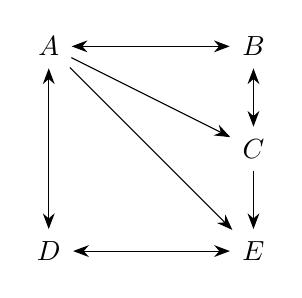
\begin{tikzpicture}[link graph]
    \node (A) at (0, 2.6) {$A$};
    \node (B) at (2.6, 2.6) {$B$};
    \node (C) at (2.6, 1.3) {$C$};
    \node (D) at (0, 0) {$D$};
    \node (E) at (2.6, 0) {$E$};
    \draw[<->] (A) -- (B);
    \draw[<->] (B) -- (C);
    \draw[->] (A) -- (C);
    \draw[->] (A) -- (E);
    \draw[<->] (A) -- (D);
    \draw[->] (C) -- (E);
    \draw[<->] (D) -- (E);
  \end{tikzpicture}
\end{center}

The PageRank algorithm assigns ranks $r(A)$, $r(B)$, $r(C)$, $r(D)$, and $r(E)$ that are all between $0$ and $1$ (inclusive) and sum to $1$.

Each page equally distributes its own PageRank along its outbound links. For example, page $B$ has two outbound links, so page $B$ ``donates'' $\frac{r(B)}{2}$ to both page $A$ and page $C$. Page $D$ also gives half its PageRank to page $A$, so the PageRank of $A$ satisfies:
\begin{align*}
  r(A) = \frac{r(B)}{2} + \frac{r(D)}{2}
\end{align*}
Since page $B$ has inbound links from page $A$ (which has four total outbound links) and page $C$ (which has two total outbound links), the PageRank of page $B$ satisfies:
\begin{align*}
  r(B) = \frac{r(A)}{4} + \frac{r(C)}{2}
\end{align*}
The full list of equations is:
\begin{align*}
  r(A) & = \frac{r(B)}{2} + \frac{r(D)}{2}                  \\[1ex]
  r(B) & = \frac{r(A)}{4} + \frac{r(C)}{2}                  \\[1ex]
  r(C) & = \frac{r(A)}{4} + \frac{r(B)}{2}                  \\[1ex]
  r(D) & = \frac{r(A)}{4} + r(E)                            \\[1ex]
  r(E) & = \frac{r(A)}{4} + \frac{r(C)}{2} + \frac{r(D)}{2}
\end{align*}
The unique solution of this system of linear equations for which the sum of the PageRanks is $1$ is:
\begin{align*}
  \begin{bmatrix}
    r(A) \\
    r(B) \\
    r(C) \\
    r(D) \\
    r(E)
  \end{bmatrix} = \begin{bmatrix}
                    0.211 \\
                    0.105 \\
                    0.105 \\
                    0.316 \\
                    0.263
                  \end{bmatrix}
\end{align*}
We always normalize our solution vector so that the sum of the PageRanks is $1$.

Interpreting these results, we see that page $D$ would show up first in a search since it has the highest rank ($0.316$), followed by page $E$, with a rank of $0.263$, and so on. It is interesting to note that even though page $E$ has the most inbound links, it doesn't have the highest PageRank. This is because page $E$ only has one outbound link, to page $D$, so page $D$ receives the entirety of page $E$'s PageRank, plus a small contribution from page $A$.

\textbf{Exercise 1}: (6 points) Use the technique of the example above to find the PageRanks of pages $A$, $B$, and $C$ in the graph below.

\begin{center}
  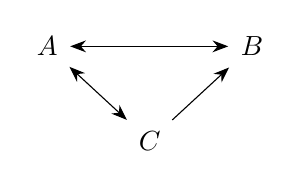
\begin{tikzpicture}[link graph]
    \node (A) at (0, 1.2) {$A$};
    \node (B) at (2.6, 1.2) {$B$};
    \node (C) at (1.3, 0) {$C$};
    \draw[<->] (A) -- (B);
    \draw[<->] (A) -- (C);
    \draw[->] (C) -- (B);
  \end{tikzpicture}
\end{center}

\textbf{Example 1 (con't)}: Returning to our example, we may write the system of linear equations we found in matrix form:
\begin{align*}
  \begin{bmatrix}
    0    & 0.5 & 0   & 0.5 & 0 \\
    0.25 & 0   & 0.5 & 0   & 0 \\
    0.25 & 0.5 & 0   & 0   & 0 \\
    0.25 & 0   & 0   & 0   & 1 \\
    0.25 & 0   & 0.5 & 0.5 & 0
  \end{bmatrix} \vec{r} = \vec{r}, \qquad \text{where } \vec{r} = \begin{bmatrix}
                                                                    r(A) \\
                                                                    r(B) \\
                                                                    r(C) \\
                                                                    r(D) \\
                                                                    r(E)
                                                                  \end{bmatrix}
\end{align*}
Denote the $5 \times 5$ matrix above by $P$. The columns of $P$ describe the outbound links from each webpage (the first column of $P$, for example, indicates that $A$ has outbound links to $B$, $C$, $D$, and $E$, and equally distributes its PageRank among them). Because of this, the sum of the entries in each column of $P$ is $1$. In other words, $P$ is a stochastic matrix, and can be thought of as the \emph{transition matrix} of a Markov chain. Additionally, the vector $\vec{r}$ of PageRanks we are searching for is an eigenvector of $P$ corresponding to the eigenvalue $\lambda = 1$. Since the entries of $\vec{r}$ sum to $1$, $\vec{r}$ is actually a steady-state vector of $P$!

This Markov connection is not accidental. Suppose we start on a random page ($A$ through $E$) and begin randomly clicking links. If $\vec{x}_0$ in $\R^5$ is the probability vector for our initial location (i.e., the components of $\vec{x}_0$ are the probabilities that we begin at page $A$, or page $B$, etc.), then $P^{50}\vec{x}_0$ is the probability vector for our location after $50$ random clicks. As we'll see later, in ``nice'' cases the sequence of vectors $P^k\vec{x}_0$ approaches the steady-state (PageRank) vector $\vec{r}$ as $k \to \infty$, no matter what $\vec{x}_0$ is. In this way, we can interpret the PageRank vector as a vector of probabilities for our location after many random clicks. In Example 1, $r(C) = 0.105$ means that if we start on a random page and click a large number of random links, then there is about a $10.5\%$ chance that our final destination is page $C$.

We'll see later that this realization makes it possible to approximate the PageRank vector in cases where it is infeasible to calculate the PageRank vector directly, but we are still left with a question: can we always frame the problem of finding PageRanks in terms of finding the steady-state vector of a related stochastic matrix? The following example will help settle the question.

\textbf{Example 2}: Consider the simple graph of links below:

\begin{center}
  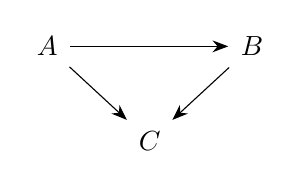
\begin{tikzpicture}[link graph]
    \node (A) at (0, 1.2) {$A$};
    \node (B) at (2.6, 1.2) {$B$};
    \node (C) at (1.3, 0) {$C$};
    \draw[->] (A) -- (B);
    \draw[->] (A) -- (C);
    \draw[->] (B) -- (C);
  \end{tikzpicture}
\end{center}

The corresponding matrix is:
\begin{align*}
  P = \begin{bmatrix}
        0   & 0 & 0 \\
        1/2 & 0 & 0 \\
        1/2 & 1 & 0
      \end{bmatrix}
\end{align*}
The third column of $P$ is the zero vector, so $P$ is \emph{not} the transition matrix of a Markov chain! If we access a random page ($A$, $B$, or $C$) and click links randomly, then we always end up stuck at $C$ after at most two clicks. To remedy this, \textbf{whenever we have a page that doesn't link to any other pages, we modify the link diagram so that the page links to \emph{all} pages, even itself.} In this example, we draw arrows from $C$ to all three pages:

\begin{center}
  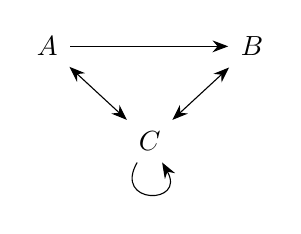
\begin{tikzpicture}[link graph]
    \node (A) at (0, 1.2) {$A$};
    \node (B) at (2.6, 1.2) {$B$};
    \node (C) at (1.3, 0) {$C$};
    \draw[->] (A) -- (B);
    \draw[<->] (A) -- (C);
    \draw[<->] (B) -- (C);
    \draw[->] (C) to[out=-120, in=-60, looseness=6] (C);
  \end{tikzpicture}
\end{center}

The new matrix is:
\begin{align*}
  \widetilde{P} = \begin{bmatrix}
                    0   & 0 & 1/3 \\
                    1/2 & 0 & 1/3 \\
                    1/2 & 1 & 1/3
                  \end{bmatrix}
\end{align*}
We call $\widetilde{P}$ the \emph{altered transition matrix}. In general, if there are $n$ webpages, then we form $\widetilde{P}$ from $P$ by replacing any columns of zeroes by the vector $(\frac{1}{n}, \frac{1}{n}, \ldots, \frac{1}{n})$. An altered transition matrix is always a stochastic matrix (why?), and should be used to find PageRanks if at least one webpage does not link to other pages.

\textbf{Exercise 2}: (12 points) Consider the link diagram below.

\begin{center}
  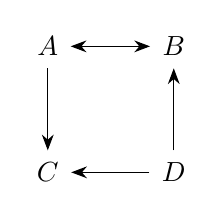
\begin{tikzpicture}[link graph]
    \node (A) at (0, 1.6) {$A$};
    \node (B) at (1.6, 1.6) {$B$};
    \node (C) at (0, 0) {$C$};
    \node (D) at (1.6, 0) {$D$};
    \draw[<->] (A) -- (B);
    \draw[->] (A) -- (C);
    \draw[->] (D) -- (B);
    \draw[->] (D) -- (C);
  \end{tikzpicture}
\end{center}

\begin{enumerate}[label=\alph*.]

  \item (4 points) Show that the method you used in Exercise 1 to find PageRanks doesn't work here. [Note that $D$ has no inbound links, so $r(D) = 0$.]

  \item (2 points) Find the altered transition matrix $\widetilde{P}$.

  \item (6 points) Find the PageRank vector by finding the unique steady-state vector of $\widetilde{P}$.

\end{enumerate}

\textbf{Exercise 3}: (8 points) Consider the very simple link diagram below. Ralph has a $\frac{2}{3}$ chance of starting at page $A$ and a $\frac{1}{3}$ chance of starting at page $B$. Once per minute, he clicks on a random link, if possible.

\begin{center}
  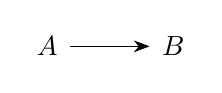
\begin{tikzpicture}[link graph]
    \node (A) at (0, 0) {$A$};
    \node (B) at (1.6, 0) {$B$};
    \draw[->] (A) -- (B);
  \end{tikzpicture}
\end{center}

\begin{enumerate}[label=\alph*.]

  \item (2 points) What is the probability that Ralph will be on page $B$ after four minutes?

  \item (6 points) Now suppose that whenever Ralph accesses page $B$, after one minute he will randomly (with equal probability) jump to either page $A$ or stay on page $B$. Find the probability that Ralph will be on page $B$ after four minutes.

\end{enumerate}

Finding a steady-state vector of an altered transition matrix works well when the number of webpages is small, but is completely unfeasible when attempting to rank millions of webpages. In such a case, the best we can do is to approximate the PageRank vector. The following definition and theorem from your text help us to do this.

\textbf{Definition}: A stochastic matrix $P$ is \emph{regular} if for some $k$ every entry of $P^k$ is positive.

\textbf{Theorem}: If $P$ is a regular stochastic matrix, then $P$ has a unique steady-state vector $\vec{r}$. Additionally, if $\vec{x}_0$ is a probability vector, then the Markov chain $\{P^k\vec{x}_0\}$ approaches $\vec{r}$ as $k \to \infty$.

\textbf{Exercise 4}: (8 points) Consider the graph of links below.

\begin{center}
  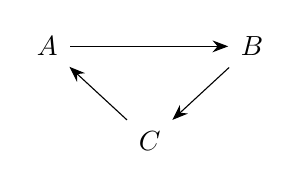
\begin{tikzpicture}[link graph]
    \node (A) at (0, 1.2) {$A$};
    \node (B) at (2.6, 1.2) {$B$};
    \node (C) at (1.3, 0) {$C$};
    \draw[->] (A) -- (B);
    \draw[->] (B) -- (C);
    \draw[->] (C) -- (A);
  \end{tikzpicture}
\end{center}

The PageRank vector is, unsurprisingly, $\vec{r} = \begin{bmatrix}
    1/3 \\
    1/3 \\
    1/3
  \end{bmatrix}$.

\begin{enumerate}[label=\alph*.]

  \item (2 points) Find the altered transition matrix $\widetilde{P}$.

  \item (4 points) Let $\vec{x}_0 = \begin{bmatrix}
            0.2 \\
            0.3 \\
            0.5
          \end{bmatrix}$. Find $\widetilde{P}\vec{x}_0$, $\widetilde{P}^2\vec{x}_0$, $\widetilde{P}^3\vec{x}_0$, and $\widetilde{P}^{100}\vec{x}_0$.

  \item (2 points) Does the sequence $\{\widetilde{P}^k\vec{x}_0\}$ approach $\vec{r}$?

\end{enumerate}

If the altered transition matrix $\widetilde{P}$ is not regular, then $\widetilde{P}$ may not have a unique steady-state vector, and the limit of a Markov chain $\{P^k\vec{x}_0\}$ may not be a steady-state vector of $\widetilde{P}$. To fix this, we build a new matrix out of $\widetilde{P}$ whose entries are all positive.

If $\widetilde{P}$ is $n \times n$, define $M$ to be the $n \times n$ matrix whose columns are all $(\frac{1}{n}, \frac{1}{n}, \ldots, \frac{1}{n})$, and let $0 < \alpha < 1$. Define the \emph{Google matrix} $G_\alpha$ as follows:
\begin{align*}
  G_\alpha = \alpha\widetilde{P} + (1 - \alpha)M
\end{align*}

\textbf{Theorem}: The Google matrix $G_\alpha$ is a stochastic matrix whose entries are all positive.

\textbf{Proof}: Since $\widetilde{P}$ was stochastic, the columns of $\widetilde{P}$ sum to $1$, so that the columns of the Google matrix sum to $\alpha \cdot 1 + (1 - \alpha) \cdot (\frac{1}{n} + \cdots + \frac{1}{n}) = \alpha + (1 - \alpha) \cdot n \cdot \frac{1}{n} = 1$.

Since $0 < \alpha < 1$, $\alpha$ and $1 - \alpha$ are positive. And since the entries of $\widetilde{P}$ were nonnegative, the entries of $G_\alpha$ have the form $(\text{pos.})(\text{nonneg.}) + (\text{pos.})(\text{pos.}) = (\text{nonneg.}) + (\text{pos.})$, and hence are positive. \hfill $\blacksquare$

The theorem implies that the Google matrix $G_\alpha$ is a regular stochastic matrix, and thus for any probability vector $\vec{x}_0$, the Markov chain $\{G_\alpha^k\vec{x}_0\}$ converges to the unique steady-state vector of $G_\alpha$. If $\alpha$ is close to $1$, then $G_\alpha$ is very close to $\widetilde{P}$, and its steady-state vector is close to a steady-state vector of $\widetilde{P}$ (assuming $\widetilde{P}$ has a unique steady-state vector, then this is the PageRank vector $\vec{r}$). If $\vec{x}_0$ is any probability vector, then for a large value of $k$, $G_\alpha^k\vec{x}_0$ should be a good approximation to the PageRank vector $\vec{r}$. The convergence of $\{G_\alpha^k\vec{x}_0\}$ to the steady-state vector of $G_\alpha$ is typically quicker for smaller values of $\alpha$, but of course for larger values of $\alpha$ the steady-state vector of $G_\alpha$ is usually closer to a steady-state vector of $\widetilde{P}$. Google hasn't publicly revealed what value of $\alpha$ it uses, but it's thought to be around $0.85$.

\textbf{Exercise 5}: (6 points) Refer back to Exercise 4.

\begin{enumerate}[label=\alph*.]

  \item (2 points) Find the Google matrix $G_{0.5}$.

  \item (2 points) Verify that in this case the steady-state vector of $G_{0.5}$ is the same as the PageRank vector $\vec{r}$.

  \item (2 points) Note that $G_{0.5}^5 \begin{bmatrix}
            0.2 \\
            0.3 \\
            0.5
          \end{bmatrix} = \begin{bmatrix}
            0.332 \\
            0.339 \\
            0.329
          \end{bmatrix}$. Explain why it's not surprising that this vector is very close to the PageRank vector $\vec{r}$.

\end{enumerate}

\pagebreak
\printbibliography

\end{document}
